\begin{surferPage}{A Double Done}
 A surface is called non-singular or smooth if it does not have any apex
    (such points are called singularities).
    Examples of smooth surfaces are a sphere or a torus (the first 2
    pictures): 
    \vspace{-0.2cm}
    \begin{center}
      \begin{tabular}{@{}c@{}c@{}c@{}c@{}}
        \begin{tabular}{@{}c}
          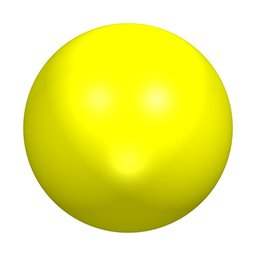
\includegraphics[width=1.1cm]{../../common/images/kugel}
        \end{tabular}
        &
        \begin{tabular}{@{}c}
          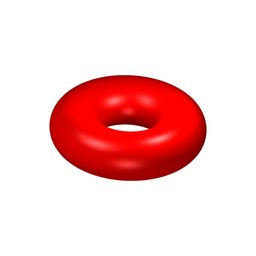
\includegraphics[width=1.1cm]{../../common/images/torus}
        \end{tabular}
        &
        \begin{tabular}{c@{}}
          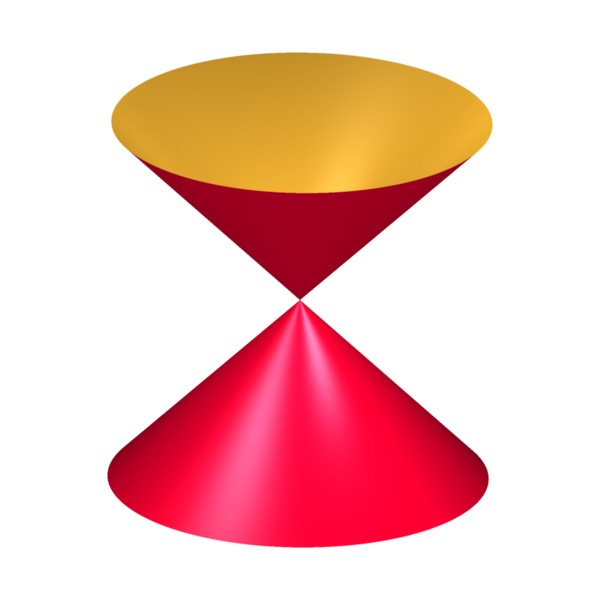
\includegraphics[width=1.1cm]{../../common/images/kegel}
        \end{tabular}
        &
        \begin{tabular}{c@{}}
          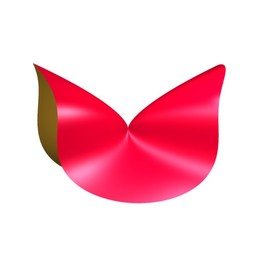
\includegraphics[width=1.1cm]{../../common/images/A2pm_ill}
        \end{tabular}
      \end{tabular}
    \end{center}
    \vspace*{-0.4em}
    The double cone (also called singularity of type $A_1^{+-}$) is the
    simplest singularity:
    when deforming the equation
    \[x^2+y^2-z^2=0\]
    slightly, it becomes smooth.
    The pictures below show surfaces corresponding to the equation
    \[x^2+y^2-z^2=a\]
    for the values $a=-\frac12$, $a=0$, $a=\frac12$:
    % 
    \begin{center}
      \vspace*{-0.4em}
      \begin{tabular}{@{}c@{\quad}c@{\quad}c@{}}
        \begin{tabular}{@{}c@{}}
          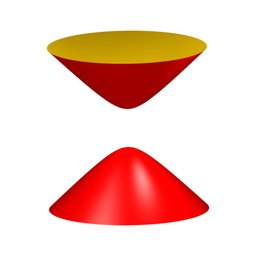
\includegraphics[width=1.2cm]{../../common/images/A1pm_0}
        \end{tabular}
        &
        \begin{tabular}{@{}c@{}}
          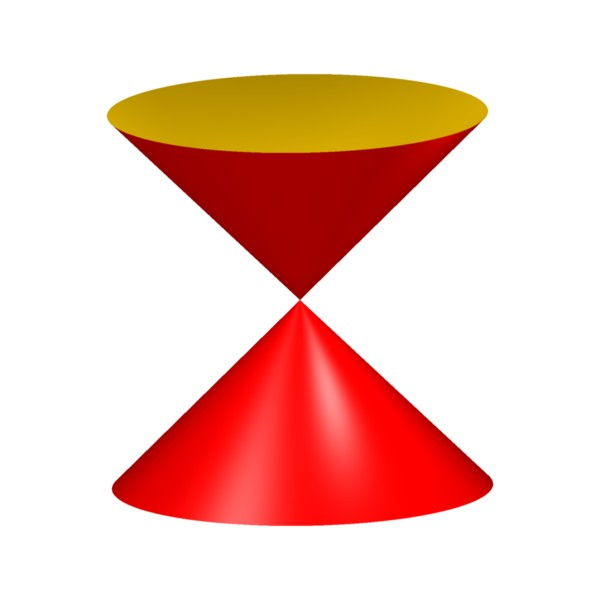
\includegraphics[width=1.2cm]{../../common/images/A1pm_1}
        \end{tabular}
        &
        \begin{tabular}{@{}c@{}}
          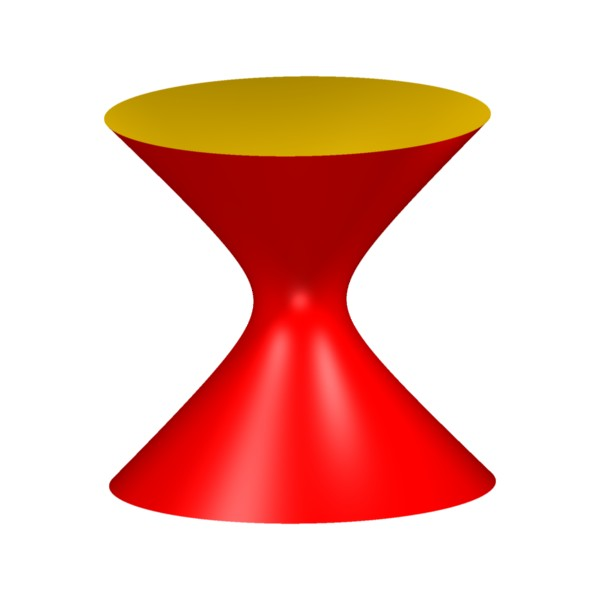
\includegraphics[width=1.2cm]{../../common/images/A1pm_2}
        \end{tabular}
      \end{tabular}
    \end{center}
    \vspace*{-0.4em}
    We will see in the following examples that it is possible to deform more
    complicated singularities in a way such that several double cones develop.
\end{surferPage}